\chapter{区块链的技术发展历程}

\section{区块链的起源与早期发展}

2008年,化名中本聪(Satoshi Nakamoto)发布了比特币的白皮书《比特币:一种点对点的电子现金系统》,提出了一种无需依赖中央银行或中介机构的去中心化数字货币。比特币的核心技术创新就是区块链(如图7.1所示),通过去中心化的分布式账本技术,确保了比特币网络中的交易能够公开透明且无法篡改。

\begin{figure}
	\centering
	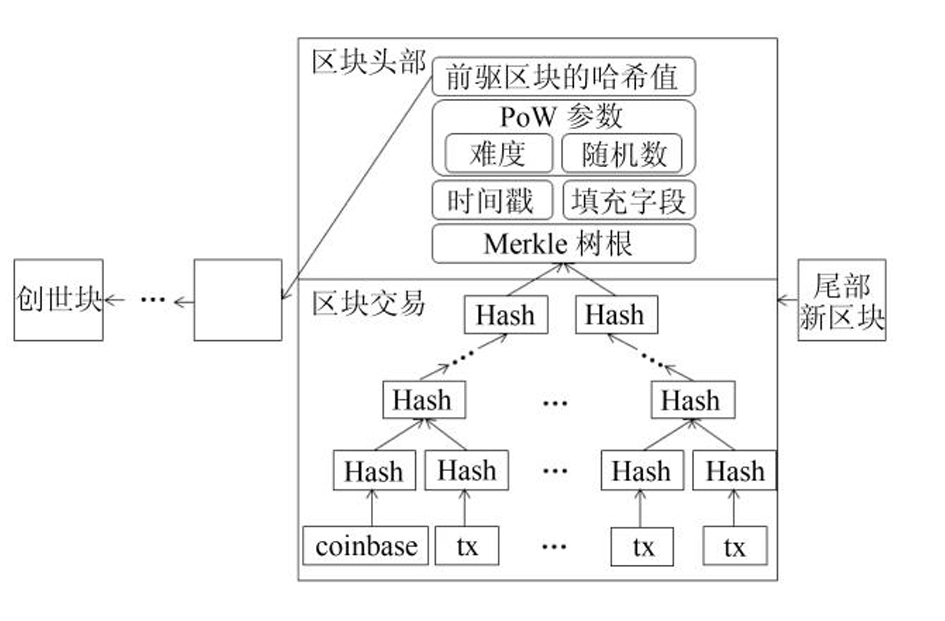
\includegraphics[width=0.5\textwidth]{img/4.png}
	\caption{比特币区块链结构}
	\label{fig:example}
\end{figure}

2009年1月,比特币的创世区块(Genesis Block)被成功挖出,标志着区块链技术的正式诞生。比特币区块链利用“工作量证明”(Proof of Work,PoW)机制保障数据的安全性和不可篡改性。

\section{关键技术突破与演进}

自从早期区块链交易之后,区块链的关键技术突破主要包括共识机制的创新(如从PoW到PoS)、智能合约的应用与优化、侧链与跨链技术的进展、隐私保护技术(如零知识证明)的发展,以及可扩展性和性能的提升(如分片技术)等。

以下从两个我感兴趣的方面入手(毫无疑问,我无法写出所有的技术突破)介绍关键技术突破与演进,即共识机制的创新(如从PoW到PoS),和零知识证明(在深圳大学区块链宣讲上提问但没有得到满意解答)。

\subsection{共识机制的创新(如从PoW到PoS)}

在PoW机制下,矿工通过计算复杂的数学难题来获得新区块的打包权(即生产新区块)。解决这些难题需要大量的计算能力和能源,矿工需要不断地进行哈希计算,直到找到一个符合要求的哈希值(称为“挖矿”)。

PoS机制通过将区块生产的权力分配给持有大量代币的用户,而不是通过算力竞赛来竞争新区块。具体来说,节点根据其持有的代币数量(或称为“股权”)来决定是否能够打包新区块。持有更多代币的人更有可能被选中创建新区块。

\subsection{隐私保护技术(如零知识证明)的发展}

零知识证明最早由\textbf{Shafi Goldwasser}、\textbf{Silvio Micali}和\textbf{Charles Rackoff}在1980年代提出。其基本思想是:证明者能够向验证者证明某个陈述是正确的,而不需要透露任何与陈述本身相关的具体信息。通过这一机制,能够保护交易、身份等敏感信息的隐私。 \\

\textbf{零知识证明的早期发展历程}

早期的ZKP(交互式零知识证明):最初的零知识证明是交互式的,证明者和验证者需要进行多轮互动才能达成验证。虽然这种方法理论上可行,但由于互动过程较为繁琐,因此难以应用到实际的区块链系统中。

非交互式零知识证明(NIZK):为了提高效率,研究人员提出了非交互式零知识证明(NIZK),其中证明者只需生成一个证明,验证者通过对该证明的验证即可确认其有效性。这种方式显著提高了零知识证明的实际应用性,并成为区块链系统中较为常见的形式。

\textbf{零知识证明的技术突破} \\
(这里仅列出零知识证明的突破,具体证明需要数理逻辑方法,这里不予列出):具体证明参见[13]  \\

•  zk-STARKs(Zero-Knowledge Scalable Transparent Arguments of Knowledge):与zk-SNARKs相比,zk-STARKs不仅提升了隐私保护能力,还增强了可扩展性和透明性。zk-STARKs不依赖于可信设置(如SNARKs中的“可信设置”),这意味着其安全性得到了进一步增强。zk-STARKs能够处理更大规模的数据集,并且适用于更加复杂的计算和证明,因此它在未来的区块链系统中有着广泛的应用前景。

•  Bulletproofs:Bulletproofs是另一种零知识证明协议,旨在提高证明的效率,尤其是针对大规模数据集的场景。Bulletproofs比zk-SNARKs更加灵活,尤其在不依赖于特殊的设置的情况下,它提供了较低的证明大小和较快的验证速度。Bulletproofs在如Monero等隐私保护加密货币中也有应用。




